\scanpage{84}
% archive foliation: 83
\figure{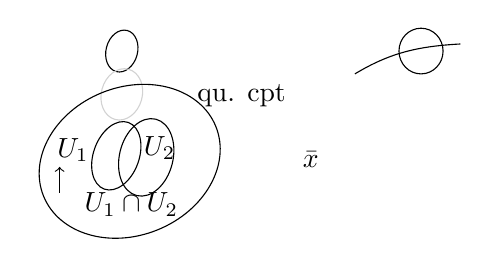
\begin{tikzpicture}[x=1cm,y=1cm]
\draw (-1.05,2.05) ellipse[x radius=.20,y radius=.27,rotate=-15];
\draw[gray!35] (-1.05,1.50) ellipse[x radius=.26,y radius=.33,rotate=-15];
\draw[rotate around={22:(-.95,.65)}] (-.95,.65) ellipse[x radius=1.18,y radius=.94];
\draw[rotate around={-20:(-1.12,.72)}] (-1.12,.72) ellipse[x radius=.29,y radius=.45];
\draw[rotate around={-14:(-.74,.70)}] (-.74,.70) ellipse[x radius=.34,y radius=.50];
\node at (-1.67,.79) {$U_1$};
\node at (-.57,.82) {$U_2$};
\node at (-.93,.10) {$U_1\cap U_2$};
\node at (.47,1.48) {\unsure{qu. cpt}};
\draw[->] (-1.84,.25)--(-1.84,.58);
\node at (1.35,.67) {$\bar x$};
\draw (2.75,2.05) ellipse[x radius=.28,y radius=.29];
\draw (1.91,1.76) .. controls (2.36,2.03) and (2.71,2.11) .. (3.25,2.14);
\end{tikzpicture}}

\figure{\begin{tikzpicture}\draw (0,0)--(6,0);\end{tikzpicture}}
\margin{\figure{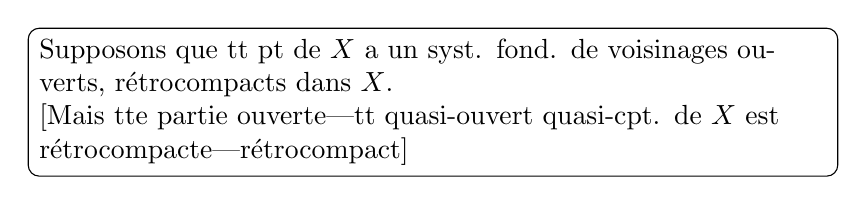
\begin{tikzpicture}
\node[draw,rounded corners=4pt,align=left,text width=10cm,inner sep=4pt] {Supposons que tt pt de $X$ a un syst. fond. de voisinages ouverts,
rétrocompacts dans $X$.\\{}
[Mais \unsure{tte partie ouverte|tt quasi-ouvert} \unsure{quasi-cpt.} de $X$ est \unsure{rétrocompacte|rétrocompact}]};
\end{tikzpicture}}}

Soit $\unsure{F|\mathcal T}$ une partie fermée irréductible de $X$.
Conditions équivalentes
\margin{\diagram{\begin{tikzcd}[ampersand replacement=\&,row sep=small]
\unsure{E} \arrow[d,no head] \\ \unsure{U}
\end{tikzcd}}}

i) Il existe une partie $Z$, ouverte non vide dans $T$,
telle que $Z$ soit constructible dans $X$

ii) Il existe un ouvert \inserted{quasi-compact} $U$ de $X$, tel que
$U\cap T\ne\varnothing$, et $U-U\cap T$ soit qu. cpt.

% Reversed typewriting is show-through from the separately supplied printed face, scan 85.
